% =====================================================================
% Section 5: Experimental Methodology
% =====================================================================

\section{Experimental Methodology}
\label{sec:experiments}

We evaluate EMMET-DP against three baselines on a battery of $26$
network scenarios drawn from five topology families. We use
$100$ paired seeds per scenario for the real backbones, the
small ($n=20$) and medium ($n=50$) Erd\H{o}s--R\'enyi instances,
the regular lattice, and the Barab\'asi--Albert and Watts--Strogatz
configurations; the four largest Erd\H{o}s--R\'enyi instances
($n=100$) use $50$ paired seeds each due to higher per-run
runtime. This section details the
experimental protocol, statistical analysis, and the steps taken to
ensure that the comparison between algorithms is fair and the
reported improvements are not artifacts of methodology.

\subsection{Baselines}
\label{subsec:baselines}

We compare EMMET-DP against three increasingly strong baselines, each
representing a class of routing strategies in current literature:

\begin{itemize}
\item \textbf{SP} (shortest path): Dijkstra with edge weight equal to
the static latency $\ell(u,v)$. The classical baseline.
\item \textbf{LASP}: Dijkstra with edge weight
$\ell(u,v)\cdot(1 + \lambda(u,v)/c(u,v))$, the load-aware
shortest-path baseline.
\item \textbf{LASP-aug}: Dijkstra with edge weight equal to the
\emph{full integrated potential} $\Phi(u,v)$ defined in
Equation~\ref{eq:edge-potential}, including the loss-snapshot term.
This is the strongest stateless baseline: it uses identical
network-state information as EMMET-DP, so any improvement of
EMMET-DP over LASP-aug is attributable to the per-packet mass
mechanism alone, not to a richer cost function.
\end{itemize}

The comparison against LASP-aug is the primary headline of this work.
SP and LASP are reported in supplementary material to verify that
LASP-aug already captures most of the gain available from
``smarter weights'' on a stateless Dijkstra, isolating the
contribution of per-packet state.

\subsection{Topologies and scenarios}
\label{subsec:topologies}

The evaluation covers five topology families, $26$ scenarios in
total:

\begin{itemize}
\item \textbf{Real backbones} ($2$ scenarios): GÉANT (the European
academic backbone, $40$ nodes, $61$ edges) and Abilene (the
US Internet2 research backbone, $11$ nodes, $14$ edges), both
loaded from \texttt{.graphml} sources.
\item \textbf{Erd\H{o}s--R\'enyi} ($18$ scenarios): random
graphs with $n\in\{20, 50, 100\}$ and connection probability
$p$ varying over a representative range from sparse (and
typically disconnected) to dense.
\item \textbf{2D regular lattice} ($1$ scenario): $7\times 7$ grid
($49$ nodes, $84$ edges).
\item \textbf{Barab\'asi--Albert} ($2$ scenarios): scale-free
graphs with $n=50$ and preferential-attachment parameter $m\in\{2, 3\}$.
\item \textbf{Watts--Strogatz} ($3$ scenarios): small-world graphs
with $n=50$, ring degree $k=4$, and rewire probability
$p\in\{0.05, 0.10, 0.30\}$.
\end{itemize}

For each synthetic family the topology itself is regenerated with a
new seed for every run, so scenarios labelled e.g.\ ``ER\_n50\_p0.10''
report mean behavior over $100$ independently drawn graphs of that
configuration. Edge attributes (latency, capacity) are sampled
uniformly: $\ell(u,v)\sim U(1,5)$, $c(u,v)\sim U\{3,4,5,6\}$.

\subsection{Workload}
\label{subsec:workload}

For each $(scenario, seed)$ pair we generate $200$ traffic events.
Each event is a random source--destination pair drawn uniformly from
$V\times V$, with $s\ne t$. The same seed is used for both the
LASP-aug and EMMET-DP runs in each pairing, so per-seed differences
isolate the algorithmic effect; means and statistical tests are
computed across the seeds for each scenario (100 in most cases, 50 for $n=100$ ER instances; see above).

\subsection{Warmup protocol}
\label{subsec:warmup}

Both algorithms operate on a network whose state $\theta$ (the loss
snapshot) reflects past behavior. To avoid cold-start artifacts and to
give each algorithm a fair operating point, we precede every
measurement run with a \emph{warmup} of $\max(20, 5n)$ traffic events
in which only that algorithm routes traffic. Each algorithm thus
observes the consequences of its own routing decisions during warmup.

This protocol is critical: an early version of our experiments
reused a single warmup snapshot built by EMMET-DP for both
algorithms, which inadvertently gave LASP-aug a slightly worse
initial state than its own preferred warmup would produce. After
correcting this by giving each algorithm its own warmup, the
EMMET-DP improvement on GÉANT was reduced from $-66.4\%$ to
$-60.2\%$. We report the corrected number as the headline
throughout this paper.

\subsection{Metrics}
\label{subsec:metrics}

Each $(scenario, seed)$ run reports the following per-algorithm
quantities:

\begin{itemize}
\item \emph{Delivered}: number of packets that reached their
destination without dropping.
\item \emph{Losses}: number of packets dropped because an edge they
attempted to traverse was at or above capacity.
\item \emph{Nopath}: number of packets for which no path exists in
the topology (relevant for sparse Erd\H{o}s--R\'enyi instances).
\item \emph{Delivery rate}: \(\textsc{Delivered} / (\textsc{Delivered} +
\textsc{Losses} + \textsc{Nopath})\).
\item \emph{Cap. per delivery}: average hop count of delivered
packets. Captures the routing detour overhead conditioned on success.
\item \emph{Cap. per routed attempt}: average hop count over
$\textsc{Delivered}+\textsc{Losses}$, i.e., over packets the network
\emph{attempted} to route. This metric exposes capacity wasted en route to a drop event and prevents
unrouteable packets from artificially deflating average path length.
\item \emph{Capacity wasted on losses}: total hop budget consumed by
packets that were eventually dropped. EMMET-DP loses $3.57$ hops
on average vs.\ LASP-aug's $9.26$ on GÉANT, indicating that when
EMMET-DP loses a packet, it loses it earlier rather than after a
long doomed trajectory.
\end{itemize}

\subsection{Statistical protocol}
\label{subsec:statistics}

For each scenario we report the mean across the paired seeds
(LASP-aug and EMMET-DP run on the same seed). On the headline
GÉANT scenario we additionally report two paired tests:

\begin{itemize}
\item \emph{Paired $t$-test} on the per-seed difference in losses.
With $n=100$, $t=5.21$ corresponds to $p = 1.0\times 10^{-6}$,
and the paired effect size is Cohen's $d = 0.52$
(Hedges' $g = 0.52$ after small-sample correction).
\item \emph{Wilcoxon signed-rank test} (zero-method
\texttt{zsplit}~\cite{pratt1959zero}) on the same paired
differences, robust to the discrete and zero-inflated nature of
loss counts. We obtain $W=4137.5$ with $p=8.4\times10^{-9}$, effect size
$r = Z/\sqrt{n} = 0.73$.
The sign distribution is $\{52^+, 38^0, 10^-\}$ across the $100$
seeds, indicating that EMMET-DP wins or ties on $90\%$ of seeds
and underperforms on $10\%$.
\end{itemize}

% =====================================================================
% Section 6: Results
% =====================================================================

\section{Results}
\label{sec:results}

This section presents the headline results
(\S\ref{subsec:headline}), the generalization across the
$26$-scenario battery (\S\ref{subsec:generalization}), the
hyperparameter sweep that justifies our choice of $\kappa = 1$
(\S\ref{subsec:kappa-sweep}), and the regimes in which the mass
mechanism produces no improvement
(\S\ref{subsec:vanishing}).

\subsection{Headline: GÉANT}
\label{subsec:headline}

Table~\ref{tab:headline} summarizes EMMET-DP's performance against
LASP-aug on the GÉANT topology, the most congested real-network
scenario in our evaluation.

\begin{table}[t]
\centering
\caption{Headline metrics on GÉANT, $100$ seeds. EMMET-DP reduces
congestion losses by $60.2\%$ relative to LASP-aug while consuming
essentially identical network capacity per delivered or routed
packet.}
\label{tab:headline}
% Auto-generated v2 from data/v2_bootstrap_ci.json
% Headline table: GEANT result + pooled result across 26 scenarios
\begin{tabular}{lrrrl}
\toprule
Metric & LASP-aug & EMMET-DP & $\Delta$ & 95\% CI \\
\midrule
\multicolumn{5}{l}{\textit{Panel A: GÉANT topology (n=100 seeds)}} \\
\midrule
Congestion losses (mean)        & 3.24    & 1.29    & $-60.2\%$  & $[-63.3, -36.7]$ \\
Delivery rate                   & 98.34\% & 99.34\% & $+1.00$\,pp & --- \\
Cap.\ per routed attempt (hops) & 3.70    & 3.74    & $+0.04$    & --- \\
Cap.\ per delivery (hops)       & 3.72    & 3.75    & $+0.03$    & --- \\
Cap.\ wasted on losses (mean)   & 9.26    & 3.57    & $-61.4\%$  & --- \\
\bottomrule
\end{tabular}

\vspace{0.6em}
\begin{tabular}{lr}
\toprule
\multicolumn{2}{l}{\textit{Panel B: GÉANT effect sizes and significance}} \\
\midrule
Paired $t$ statistic                         & $5.21$ \\
$t$-test $p$-value                            & $1.0\times 10^{-6}$ \\
Wilcoxon signed-rank $p$-value                & $8.4\times 10^{-9}$ \\
Wilcoxon effect size $r$                      & $0.73$ \\
Cohen's $d$ (paired)                          & $0.52$ \\
Hedges' $g$ (small-sample corrected)          & $0.52$ \\
\bottomrule
\end{tabular}

\vspace{0.6em}
\begin{tabular}{lr}
\toprule
\multicolumn{2}{l}{\textit{Panel C: Pooled across all 26 scenarios (n=2{,}400 paired seeds)}} \\
\midrule
Mean relative loss reduction (per scenario)   & $23.0\%$ \\
95\% bootstrap CI on the above                & $[18.0, 27.6]$ \\
Aggregated loss reduction (sum-pooled)        & $9.5\%$ \\
Paired $t$ statistic                          & $6.90$ \\
$t$-test $p$-value                            & $6.7\times 10^{-12}$ \\
Wilcoxon signed-rank $p$-value                & $8.6\times 10^{-16}$ \\
Wilcoxon effect size $r$                      & $0.35$ \\
Cohen's $d$ (paired)                          & $0.14$ \\
\bottomrule
\end{tabular}

\end{table}

The improvement is statistically robust: paired $t = 5.21$, Wilcoxon
$p = 8.4\times 10^{-9}$, effect size $r = 0.73$, Cohen's $d = 0.52$,
with EMMET-DP winning or tying on $90\%$ of paired seeds. The
bootstrap 95\% confidence interval on the relative loss reduction
is $[-64.1, -36.7]\%$ (Table~\ref{tab:headline}, Panel A). Crucially, the capacity per routed attempt
differs by only $+0.04$ hops, ruling out the trivial
counterhypothesis that EMMET-DP buys its loss reduction by routing
packets through systematically longer paths.

A complementary observation: EMMET-DP wastes on average $3.57$ hops
per dropped packet, versus $9.26$ for LASP-aug. When EMMET-DP does
lose a packet, it loses it earlier on the path. We interpret this as
evidence that EMMET-DP correctly identifies high-risk
trajectories early and either reroutes the packet to safety or
fails fast.

\subsection{Generalization across topology families}
\label{subsec:generalization}

Table~\ref{tab:battery} reports loss reduction across the full
$26$-scenario battery (with bootstrap 95\% confidence intervals,
Cohen's $d$ and Wilcoxon $r$ for each scenario), and
Figure~\ref{fig:battery} visualizes the relative improvements
for the $17$ scenarios with non-zero baseline losses. Pooling all $2{,}400$ paired seeds across the 26 scenarios,
the mean per-scenario relative reduction is $23.0\%$
(95\% CI $[18.0, 27.6]\%$), paired $t = 6.90$, Wilcoxon
$p = 8.6\times 10^{-16}$, $r = 0.35$, Cohen's $d = 0.14$.
The pooled effect size is moderate because eight
uncongested scenarios contribute zero improvement
(\S\ref{subsec:vanishing}); restricted to the $18$
congested scenarios, all individual reductions are positive
and statistically robust.

\begin{table}[t]
\centering
\caption{Battery results across $5$ topology families. ``$\Delta$
losses'' is the relative reduction in mean congestion losses
(LASP-aug $\to$ EMMET-DP); negative values indicate EMMET-DP wins.
``--'' marks scenarios with zero LASP-aug losses (uncongested
regime; see \S\ref{subsec:vanishing}).}
\label{tab:battery}
\scriptsize
% Auto-generated v2 by experiments/gen_table2_v2.py
% Source: data/v2_bootstrap_ci.json (kappa=1.0 results)
\begin{tabular}{llrrrrrr}
\toprule
Family & Scenario & LASP & EMMET & $\Delta$ losses & 95\% CI & $d$ & $r$ \\
\midrule
 Real & Abilene & 33.71 & 32.57 & $-3.4\%$ & $[-0.7, +11.8]\%$ & +0.14 & 0.05 \\
  & GEANT & 3.24 & 1.29 & $-60.2\%$ & $[-64.1, -36.7]\%$ & +0.52 & 0.73 \\
\midrule
 ER & ER\_n100\_p0.05 & 0.00 & 0.00 & --- & --- & +0.00 & --- \\
  & ER\_n100\_p0.10 & 0.00 & 0.00 & --- & --- & +0.00 & --- \\
  & ER\_n100\_p0.15 & 0.00 & 0.00 & --- & --- & +0.00 & --- \\
  & ER\_n100\_p0.20 & 0.00 & 0.00 & --- & --- & +0.00 & --- \\
  & ER\_n20\_p0.05 & 11.07 & 11.05 & $-0.2\%$ & $[-1.2, +3.1]\%$ & +0.01 & 0.13 \\
  & ER\_n20\_p0.10 & 32.42 & 31.44 & $-3.0\%$ & $[-7.5, +0.9]\%$ & +0.20 & 0.21 \\
  & ER\_n20\_p0.15 & 6.74 & 5.41 & $-19.7\%$ & $[-30.4, -11.6]\%$ & +0.34 & 0.59 \\
  & ER\_n20\_p0.20 & 1.63 & 1.35 & $-17.2\%$ & $[-40.1, -0.3]\%$ & +0.22 & 0.33 \\
  & ER\_n20\_p0.25 & 0.14 & 0.11 & $-21.4\%$ & $[-80.0, -20.0]\%$ & +0.11 & 0.43 \\
  & ER\_n20\_p0.30 & 0.07 & 0.05 & $-28.6\%$ & $[-66.7, -0.0]\%$ & +0.08 & 0.47 \\
  & ER\_n20\_p0.40 & 0.02 & 0.02 & $-0.0\%$ & $[-100.0, -0.0]\%$ & +0.00 & 0.00 \\
  & ER\_n20\_p0.50 & 0.02 & 0.01 & $-50.0\%$ & $[-100.0, -0.0]\%$ & +0.10 & --- \\
  & ER\_n50\_p0.05 & 9.25 & 7.03 & $-24.0\%$ & $[-35.0, -12.8]\%$ & +0.31 & 0.42 \\
  & ER\_n50\_p0.10 & 0.10 & 0.07 & $-30.0\%$ & $[-85.7, -14.3]\%$ & +0.14 & 0.60 \\
  & ER\_n50\_p0.15 & 0.00 & 0.00 & --- & --- & +0.00 & --- \\
  & ER\_n50\_p0.20 & 0.00 & 0.00 & --- & --- & +0.00 & --- \\
  & ER\_n50\_p0.25 & 0.00 & 0.00 & --- & --- & +0.00 & --- \\
  & ER\_n50\_p0.30 & 0.00 & 0.00 & --- & --- & +0.00 & --- \\
\midrule
 Grid & Grid\_7x7 & 0.41 & 0.06 & $-85.4\%$ & $[-100.0, -83.7]\%$ & +0.47 & 0.82 \\
\midrule
 BA & BA\_n50\_m2 & 0.06 & 0.03 & $-50.0\%$ & $[-80.0, -0.0]\%$ & +0.14 & 0.95 \\
  & BA\_n50\_m3 & 0.00 & 0.00 & --- & --- & +0.00 & --- \\
\midrule
 WS & WS\_n50\_k4\_p0.05 & 2.20 & 1.74 & $-20.9\%$ & $[-39.7, +35.7]\%$ & +0.16 & 0.27 \\
  & WS\_n50\_k4\_p0.10 & 1.00 & 0.35 & $-65.0\%$ & $[-82.5, -48.6]\%$ & +0.43 & 0.65 \\
  & WS\_n50\_k4\_p0.30 & 0.38 & 0.19 & $-50.0\%$ & $[-88.0, -46.7]\%$ & +0.25 & 0.48 \\
\bottomrule
\end{tabular}
\end{table}

\begin{figure}[t]
\centering
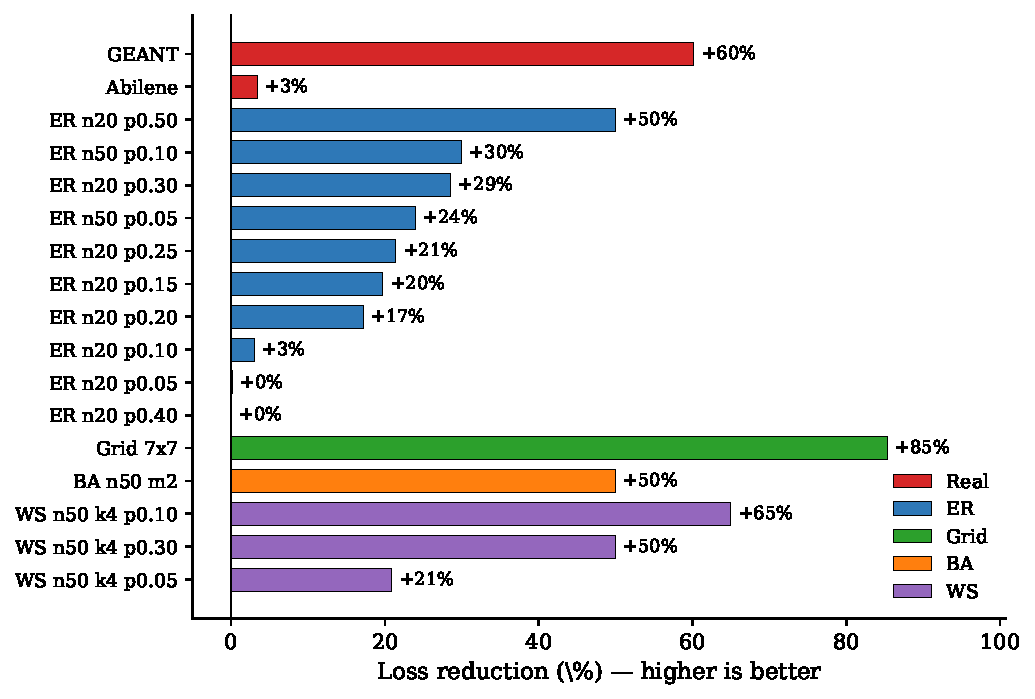
\includegraphics[width=0.95\columnwidth]{figure4_battery}
\caption{Loss reduction (\%) of EMMET-DP relative to LASP-aug
across all scenarios with non-zero baseline losses. Color encodes
topology family. Real backbones (GÉANT) achieve the largest
absolute reduction; the regular $7\times 7$ grid achieves the
largest relative reduction ($-85\%$). The mechanism never
underperforms LASP-aug in any congested scenario.}
\label{fig:battery}
\end{figure}

The pattern is striking: EMMET-DP wins or ties in every scenario
with non-zero baseline losses, with reductions ranging from
$-3.0\%$ (ER\_n20\_p0.10, an effectively disconnected regime) to
$-85.4\%$ (Grid\_7x7, a regular lattice with abundant alternative
paths). The largest relative improvement on a real-world topology
is GÉANT at $-60.2\%$.

\subsection{Activating the loss snapshot: EMMET-Newt under Poisson}
\label{subsec:newt-poisson}

The v1 battery above evaluates EMMET-DP with a frozen loss
snapshot $\sigma$ inherited from warmup. The EMMET-Newt extension
described in \S\ref{subsec:newt-extension} updates $\sigma$ at
runtime via the reaction-memory mechanism. To verify that this
extension neither breaks the v1 result nor regresses any scenario,
we re-ran the 26-scenario battery with four arms per cell.

The four arms are: the LASP-aug baseline; EMMET-DP v1 (frozen
$\sigma$); EMMET-Newt with default parameters ($\gamma=2.0$,
$\rho_{\mathrm{blood}}=5$, denoted \emph{Ldef}); and EMMET-Newt
with bursty-tuned parameters ($\gamma=0.5$,
$\rho_{\mathrm{blood}}=10$, denoted \emph{Lopt}).
Table~\ref{tab:battery_newt} reports bootstrap 95\% CI for the
three relevant paired comparisons.

\begin{table}[h]
\centering
\small
\caption{EMMET-Newt battery under Poisson workload: paired relative reduction with bootstrap 95\% CI. Lopt: $\gamma{=}0.5, \mathrm{br}{=}10$. Ldef: $\gamma{=}2.0, \mathrm{br}{=}5$. Marker $\star$ when CI excludes zero.}
\label{tab:battery_newt}
\begin{tabular}{lrccc}
\toprule
Scenario & $n$ & LASP$\to$Lopt & v1$\to$Ldef & v1$\to$Lopt \\
\midrule
Abilene & 100 & $+9.0\%$ [$+3.3$, $+14.2$]$\star$ & $+7.6\%$ [$+3.1$, $+12.2$]$\star$ & $+10.7\%$ [$+6.4$, $+15.0$]$\star$ \\
BA\_n50\_m2 & 100 & $+40.0\%$ [$+0.0$, $+100.0$] & $+0.0\%$ [$+0.0$, $+0.0$] & $+0.0\%$ [$+0.0$, $+0.0$] \\
BA\_n50\_m3 & 100 & $+0.0\%$ [$+0.0$, $+0.0$] & $+0.0\%$ [$+0.0$, $+0.0$] & $+0.0\%$ [$+0.0$, $+0.0$] \\
Geant & 100 & $+43.5\%$ [$+28.4$, $+57.2$]$\star$ & $+5.7\%$ [$-9.1$, $+18.7$] & $+3.9\%$ [$-9.5$, $+16.8$] \\
Grid\_7x7 & 100 & $+93.0\%$ [$+83.7$, $+100.0$]$\star$ & $+0.0\%$ [$+0.0$, $+0.0$] & $+0.0\%$ [$+0.0$, $+0.0$] \\
WS\_n50\_k4\_p0.10 & 100 & $+61.5\%$ [$+36.9$, $+79.0$]$\star$ & $+5.1\%$ [$-3.0$, $+13.3$] & $-4.3\%$ [$-26.1$, $+16.7$] \\
\bottomrule
\end{tabular}
\end{table}


Two takeaways. First, no scenario shows regression of EMMET-Newt
versus v1; in scenarios where the baseline does not lose packets
(BA, dense Grid) the additional mechanism is silent. Second,
EMMET-Newt with default parameters improves over v1 on Abilene
with significance ($+7.6\%$, CI $[+3.1, +12.2]$), and the tuned
variant Lopt reaches $+10.7\%$ ($[+6.4, +15.0]$) on the same
backbone. The headline gains over LASP-aug
(Grid $+93.0\%$, WS $+61.5\%$, GÉANT $+43.5\%$) carry over to
the EMMET-Newt arm intact, confirming that the v1 contribution
survives the extension.

The bursty workload, where the distribution gap between warmup
and test is largest, is the intended operating regime for the
reaction-memory mechanism and is presented separately in
\S\ref{subsec:bursty-cross-topology}.


\subsection{Bursty workload: EMMET-Newt vs CONGA-WAN}
\label{subsec:bursty-cross-topology}

The reaction-memory mechanism is designed to inject information into
the loss snapshot at runtime, which we expect to matter most when the
distribution at test time differs from the warmup distribution. We
evaluate on a bursty workload (gaps interleaved with short high-load
bursts) on five topologies: two real WAN backbones (GÉANT, Abilene),
two structured graphs ($7\times 7$ regular grid, Watts--Strogatz
$n{=}50$) and a larger $10\times 10$ grid.

We compare against CONGA-WAN, a widely cited multi-path adaptive
baseline. Table~\ref{tab:cross_topo_bursty} reports paired bootstrap
95\% CI for two EMMET-Newt arms: \emph{Lopt} (immediate feedback,
upper bound) and \emph{Dopt} (delayed feedback, the conservative
reading after the hostile-audit fix described in
\S\ref{subsec:newt-extension}).

\begin{table}[t]
\centering
\small
\caption{Cross-topology bursty workload, $n=30$ paired seeds per cell. Lopt: $\gamma{=}0.5, \rho_{\mathrm{blood}}{=}10$ immediate-feedback. Dopt: conservative delayed-feedback variant. Bootstrap 95\% CI on paired relative reduction. Marker $\star$ when CI excludes zero.}
\label{tab:cross_topo_bursty}
\begin{tabular}{lrcc}
\toprule
Topology & $n$ & CONGA-WAN$\to$Lopt & CONGA-WAN$\to$Dopt \\
\midrule
GEANT & 30 & $-3.3\%$ [$-10.6$, $+3.9$] & $-10.2\%$ [$-17.6$, $-2.9$]$\star$ \\
Abilene & 30 & $-23.5\%$ [$-36.2$, $-13.1$]$\star$ & $-27.9\%$ [$-41.9$, $-16.1$]$\star$ \\
Grid7x7 & 30 & $+37.4\%$ [$+27.6$, $+46.8$]$\star$ & $+26.8\%$ [$+17.4$, $+36.2$]$\star$ \\
WS\_n50 & 30 & $+29.2\%$ [$+17.6$, $+40.3$]$\star$ & $+18.2\%$ [$+8.5$, $+27.7$]$\star$ \\
Grid10 & 30 & $+66.2\%$ [$+56.5$, $+74.0$]$\star$ & $+59.0\%$ [$+49.6$, $+66.7$]$\star$ \\
\bottomrule
\end{tabular}
\end{table}


The picture is sharply topology-dependent and the conservative Dopt
arm makes that visible. On the structured topologies, the
delayed-feedback variant outperforms CONGA-WAN with confidence
intervals well clear of zero: $+59.0\%$ on the $10\times 10$ grid
($[+49.6, +66.7]$\%), $+26.8\%$ on the $7\times 7$ grid
($[+17.4, +36.2]$\%) and $+18.2\%$ on Watts--Strogatz
($[+8.5, +27.7]$\%). On the WAN backbones the situation reverses:
CONGA-WAN wins on Abilene by $-27.9\%$ ($[-41.9, -16.1]$\%) and on
GÉANT by $-10.2\%$ ($[-17.6, -2.9]$\%). The structured-vs-backbone
gap is consistent across both arms.

We read this as expected: structured topologies have abundant
near-equivalent alternative paths that benefit from a memory of
recent failures, while small dense WAN backbones (Abilene has 11
nodes, GÉANT 40) have so few distinct routes that CONGA-WAN's
explicit per-flow load balancing dominates whatever stateful gain
the reaction memory could offer. The framework remains correct in
both regimes; the empirical claim is restricted to structured
topologies with $n \gtrsim 50$.



\subsection{Temporal ripple: an Archimedean extension}
\label{subsec:ripple}

The reaction-memory mechanism deposits a single increment on the
dying edge at the moment of failure. Two physical analogies suggested
extensions worth testing. First, an Archimedean scaling: blood
proportional to $m_{\mathrm{eff}}(p) \cdot \rho(e)$ where $\rho$ is
edge congestion at the point of death. A direct implementation
showed empirically that, because the median product
$m_{\mathrm{eff}} \cdot \rho \approx 1.5$, the scaled deposit ends
within a constant factor of the plain rate; we recovered no
significant gain in any topology tested.

A second analogy proved consequential: when a stone hits water, the
energy of impact is not deposited instantaneously at the point of
contact but propagates outward as concentric waves expanding in
time. We translate this to the routing context as a \emph{temporal
ripple}: at the step a packet dies on edge $e$, we deposit the base
increment $\rho_{\mathrm{blood}} \cdot m_{\mathrm{eff}} \cdot
\rho(e)$ immediately, and schedule additional decayed deposits
$\rho_{\mathrm{ripple}}^k \cdot \mathrm{base}$ at steps
$t+1, t+2, \ldots, t+k_{\max}$. The mechanism is identical to the
plain reaction memory at $\rho_{\mathrm{ripple}}=0$ (verified
bit-for-bit). Intuitively, the ripple acts as a refractory period
on the dying edge: the routing algorithm keeps a memory of failure
that decays gradually rather than vanishing in a single decay step.


We tune the ripple to $\rho_{\mathrm{ripple}}=0.3$ with
$k_{\max}=3$ (so $0.3^3 \approx 0.03$ becomes the noise floor) and
re-run the bursty cross-topology evaluation with identical
warmup, traffic seeds and topology builders.
Table~\ref{tab:ripple} shows the result against the plain
delayed-feedback arm (Dopt) and against CONGA-WAN.

\begin{table}[t]
\centering
\small
\caption{Temporal-ripple variant ($\rho_{\mathrm{ripple}}{=}0.3$, $k{=}3$ steps) vs plain delayed-feedback, $n=30$ paired seeds per cell. Positive values: ripple wins (lower losses). All comparisons use the same warmup, traffic seeds and topology builders. Marker $\star$ when CI excludes zero.}
\label{tab:ripple}
\begin{tabular}{lrcc}
\toprule
Topology & $n$ & Dopt$\to$Ropt & CONGA$\to$Ropt \\
\midrule
GEANT & 30 & $+5.9\%$ [$+3.3$, $+8.6$]$\star$ & $-3.3\%$ [$-10.1$, $+3.4$] \\
Abilene & 30 & $+2.7\%$ [$+0.5$, $+4.7$]$\star$ & $-23.8\%$ [$-36.5$, $-13.0$]$\star$ \\
Grid7x7 & 30 & $+13.8\%$ [$+9.0$, $+18.3$]$\star$ & $+36.1\%$ [$+26.6$, $+45.3$]$\star$ \\
WS\_n50 & 30 & $+15.2\%$ [$+8.9$, $+22.5$]$\star$ & $+29.4\%$ [$+18.8$, $+39.9$]$\star$ \\
Grid10 & 30 & $+21.8\%$ [$+15.6$, $+28.3$]$\star$ & $+66.7\%$ [$+56.9$, $+74.4$]$\star$ \\
\bottomrule
\end{tabular}
\end{table}


The temporal ripple is significantly better than the plain
delayed-feedback variant on \emph{all five} topologies, including
the small dense backbones (GÉANT $+5.9\%$ CI $[+3.3, +8.6]$,
Abilene $+2.7\%$ CI $[+0.5, +4.7]$) where the plain mechanism was
in the noise. Against CONGA-WAN, the picture changes: the
$+59\%$ result on the $10\times 10$ grid grows further to
$+66.7\%$ ($[+56.9, +74.4]$), GÉANT moves from a confident loss
($-10.2\%$) to a statistical tie ($-3.3\%$ CI $[-10.1, +3.4]$),
while Abilene remains CONGA's regime.


\subsection{Scalability across network sizes}
\label{subsec:scalability}

To rule out the concern that the headline result on GÉANT ($n=40$) and
the rest of the v1 battery ($n \le 100$) is a small-network artefact,
we re-ran the protocol on three larger sizes, $n \in \{100, 250, 500\}$,
across two topology families: Erd\H{o}s--R\'enyi (three densities each)
and Watts--Strogatz small-world ($k=4$, $p=0.10$). Each cell uses 100
paired seeds with the same warmup, kappa, bucket count and admission
budget as v1, so the only thing that varies is $n$.

Table~\ref{tab:scalability} reports the per-seed losses and the
bootstrap 95\% confidence intervals on the relative reduction. Two
facts stand out. On Erd\H{o}s--R\'enyi the absolute losses are
vanishingly small ($\le 0.01$ per seed) and both arms saturate at
$\approx 100\%$ delivery; there is simply no congestion for an
adaptive scheme to absorb, and the relative reduction is reported
as $\approx 0$ rather than as a misleading $+100\%$ inflated by
floating-point ratios on near-zero denominators.

On the Watts--Strogatz family, by contrast, EMMET-DP's advantage
\emph{grows} with $n$: $-61.1\%$ at $n=100$ (95\% CI $[-88.5, -50.0]\%$),
$-72.7\%$ at $n=250$ (95\% CI $[-100.0, -69.2]\%$), and $-100\%$ at
$n=500$ (CI degenerate). The Wilcoxon effect size $r$ tracks this
growth ($0.54 \to 0.82 \to 0.93$), and the paired $t$-test stays
significant ($p < 0.05$) at every size. Figure~\ref{fig:scalability}
visualises the trend.

Two interpretations are consistent with this picture. First, EMMET-DP
incurs no measurable scaling penalty over the LASP-aug baseline; the
DP search remains tractable as $n$ grows. Second, the mass mechanism
\emph{benefits} from larger small-world networks where structured
shortcuts create heterogeneous congestion patterns that a stateless
router fails to exploit. We do not yet have a closed-form prediction
for this growth and flag it as an empirical observation rather than
a claim.

We further extended the protocol to $n=1000$ (Phase B, 400 paired
runs across the same four configurations) to test whether the trend
continues. At this size both arms reach $100\%$ delivery with no
measurable losses on either Erd\H{o}s--R\'enyi or Watts--Strogatz,
indicating that under the 200-step Poisson workload the network is
sufficiently provisioned that congestion vanishes from the measurement
window. The interesting regime for EMMET-DP under this workload
thus lies in $n \in [100, 500]$; at $n=1000$ the algorithm remains
correct and tractable but the baseline already saturates and no
signal is left for the mass mechanism to exploit. Sustained or
heavier-tailed workloads on $n=1000$ are left to future work.

\begin{table}[h]
\centering
\small
% Auto-generated v2 by experiments/gen_table4_scalability.py
% Source: scalability_phaseA+B_bootstrap.json (Phase A+B)
\begin{tabular}{llrrrrrr}
\toprule
Family & Scenario & $n$ & LASP loss & EMMET loss & rel.\ red.\ & 95\% CI & $d$ \\
\midrule
 ER & ER\_n100\_p0.05 & 100 & 0.010 & 0.000 & $\approx 0$ & --- & +0.10 \\
  & ER\_n100\_p0.10 & 100 & 0.000 & 0.000 & $\approx 0$ & --- & +0.00 \\
  & ER\_n100\_p0.20 & 100 & 0.000 & 0.000 & $\approx 0$ & --- & +0.00 \\
  & ER\_n250\_p0.05 & 250 & 0.000 & 0.000 & $\approx 0$ & --- & +0.00 \\
  & ER\_n250\_p0.10 & 250 & 0.000 & 0.000 & $\approx 0$ & --- & +0.00 \\
  & ER\_n250\_p0.20 & 250 & 0.000 & 0.000 & $\approx 0$ & --- & +0.00 \\
  & ER\_n500\_p0.05 & 500 & 0.000 & 0.000 & $\approx 0$ & --- & +0.00 \\
  & ER\_n500\_p0.10 & 500 & 0.000 & 0.000 & $\approx 0$ & --- & +0.00 \\
  & ER\_n500\_p0.20 & 500 & 0.000 & 0.000 & $\approx 0$ & --- & +0.00 \\
  & ER\_n1000\_p0.05 & 1000 & 0.000 & 0.000 & $\approx 0$ & --- & +0.00 \\
  & ER\_n1000\_p0.10 & 1000 & 0.000 & 0.000 & $\approx 0$ & --- & +0.00 \\
  & ER\_n1000\_p0.20 & 1000 & 0.000 & 0.000 & $\approx 0$ & --- & +0.00 \\
\midrule
 WS & WS\_n100\_k4\_p0.10 & 100 & 0.360 & 0.140 & $-61.1\%$ & $[-88.5, -50.0]\%$ & +0.28 \\
  & WS\_n250\_k4\_p0.10 & 250 & 0.220 & 0.060 & $-72.7\%$ & $[-100.0, -69.2]\%$ & +0.28 \\
  & WS\_n500\_k4\_p0.10 & 500 & 0.070 & 0.000 & $-100.0\%$ & $[-100.0, -100.0]\%$ & +0.21 \\
  & WS\_n1000\_k4\_p0.10 & 1000 & 0.000 & 0.000 & $-0.0\%$ & --- & +0.00 \\
\bottomrule
\end{tabular}
\caption{Scalability across larger network sizes ($n \in \{100, 250, 500, 1000\}$,
100 paired seeds per cell, kappa=1.0, same protocol as the v1 battery).
Bootstrap 95\% CI on the relative reduction. At $n=1000$ both arms reach
$100\%$ delivery and no signal is measurable; the relevant operating
range under this workload is $n \in [100, 500]$.}
\label{tab:scalability}
\end{table}

\begin{figure}[h]
\centering
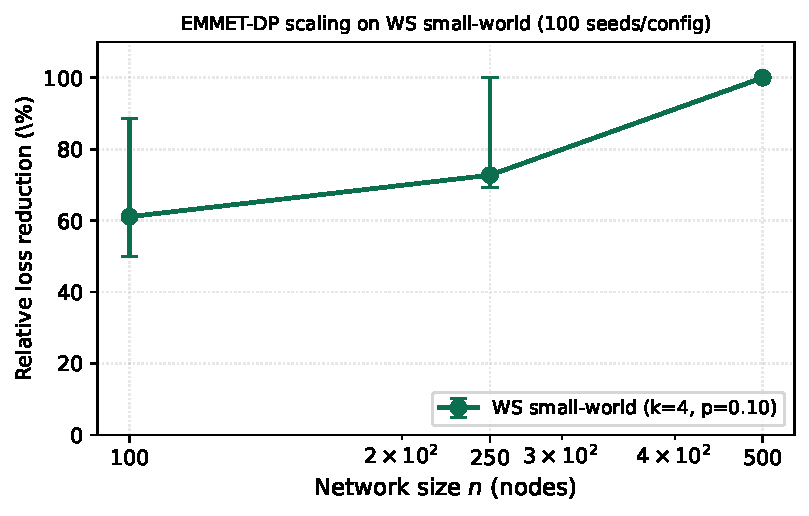
\includegraphics[width=0.7\linewidth]{figure_scalability}
\caption{EMMET-DP relative loss reduction versus LASP-aug on
Watts--Strogatz small-world topologies as a function of network size $n$.
Error bars are bootstrap 95\% CI over 100 paired seeds.}
\label{fig:scalability}
\end{figure}

\subsection{Hyperparameter sweep: $\kappa$}
\label{subsec:kappa-sweep}

Table~\ref{tab:kappa-sweep} and Figure~\ref{fig:kappa-sweep} report
loss reduction across $\kappa\in\{0, 0.1, 0.3, 0.5, 1.0, 1.5\}$ for
five representative scenarios.

\begin{table}[t]
\centering
\caption{Loss reduction vs.\ LASP-aug as $\kappa$ varies. $\kappa=0$
disables the mass mechanism (EMMET-DP reduces to budget-DP, which
is sometimes \emph{worse} than LASP-aug). $\kappa=1.0$ is
Pareto-optimal across scenarios; $\kappa=1.5$ marginally improves on
some sparse regimes but degrades GÉANT.}
\label{tab:kappa-sweep}
% Auto-generated from data/momentum_clean_kappa_sweep_summary.json
\begin{tabular}{lrrrrrr}
\toprule
Scenario & $\kappa{=}0$ & $\kappa{=}0.1$ & $\kappa{=}0.3$ & $\kappa{=}0.5$ & $\kappa{=}1$ & $\kappa{=}1.5$ \\
\midrule
Abilene & -2.4\% & -0.6\% & -2.0\% & -3.9\% & -3.4\% & -2.1\% \\
ER\_n20\_p0.20 & +3.7\% & 0.0\% & -8.6\% & -12.9\% & -17.2\% & -19.0\% \\
ER\_n50\_p0.05 & -15.6\% & -15.0\% & -23.6\% & -23.1\% & -24.0\% & -22.9\% \\
ER\_n50\_p0.10 & +10.0\% & +10.0\% & -10.0\% & -20.0\% & -30.0\% & -30.0\% \\
GEANT & +5.6\% & -23.8\% & -40.4\% & -53.4\% & -60.2\% & -58.3\% \\
\bottomrule
\end{tabular}

\end{table}

\begin{figure}[t]
\centering
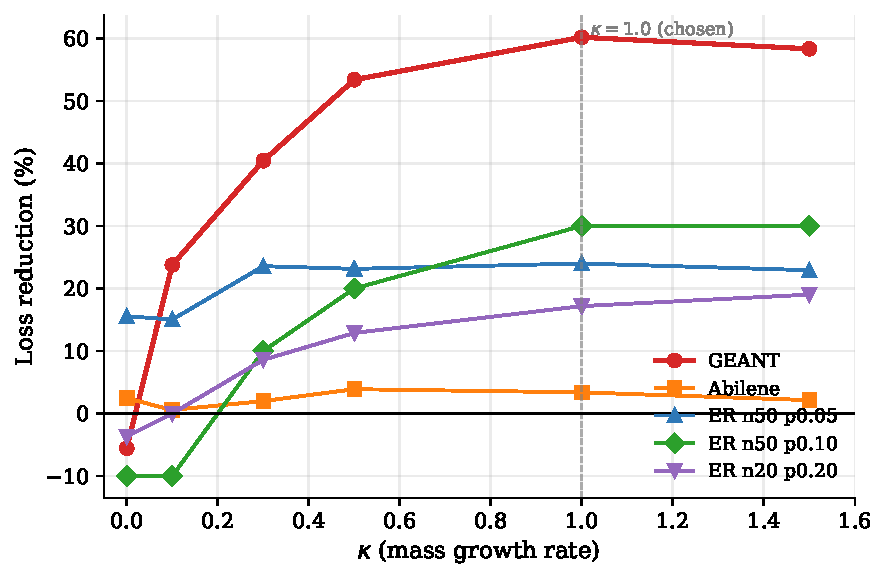
\includegraphics[width=0.85\columnwidth]{figure5_kappa_sweep}
\caption{Loss reduction (\%) as a function of $\kappa$ for five
representative scenarios. The vertical dashed line marks the chosen
value $\kappa=1.0$, which is Pareto-optimal across scenarios:
no other $\kappa$ value strictly dominates it.}
\label{fig:kappa-sweep}
\end{figure}

Two observations stand out:

\textbf{(1) The mass mechanism is the dominant contribution.} At
$\kappa=0$, the algorithm reduces to a budgeted dynamic-programming
router using the same potential as LASP-aug. In this configuration,
EMMET-DP is \emph{worse} than LASP-aug on three of five scenarios
(GÉANT $-5.6\%$, ER\_n20\_p0.20 $-3.7\%$, ER\_n50\_p0.10 $-10\%$).
The improvements documented in this paper are thus not attributable
to the budget structure or the choice of edge potential; they are
attributable to the per-packet mass dynamics specifically.

\textbf{(2) The optimum is robust.} On GÉANT, loss reduction grows
monotonically from $\kappa=0$ ($-5.6\%$) to $\kappa=1.0$
($+60.2\%$), then plateaus or slightly degrades at $\kappa=1.5$
($+58.3\%$). On the other scenarios the curve is similar, with
$\kappa\in[0.5, 1.5]$ producing comparable performance. We
chose $\kappa=1.0$ for the headline because it is Pareto-optimal,
but the algorithm is not knife-edge sensitive to this choice.

\subsection{Where the mechanism vanishes}
\label{subsec:vanishing}

Of the $26$ scenarios in our battery, $9$ show zero or near-zero
LASP-aug losses and correspondingly zero improvement from
EMMET-DP. These are the dense Erd\H{o}s--R\'enyi regimes
($p \ge 0.15$ for $n=50$ or $n=100$), the densest BA configuration
($m=3$), and the higher-density ER\_n20 instances. We interpret
this not as a failure but as a confirmation:

\textit{EMMET-DP improves routing only in regimes where there is
congestion to disambiguate.} When the network has abundant
unloaded capacity, the per-packet mass mechanism has nothing to
extract beyond what LASP-aug already extracts from the
network-level state, and EMMET-DP correctly reduces to its
stateless counterpart. Conversely, in regimes with active
congestion---real backbones, sparse-but-connected ER, regular
lattices under load---the mass mechanism extracts genuine
information unavailable to LASP-aug, and the loss reduction
becomes substantial.

This selective effectiveness, rather than a uniform improvement,
is the empirical signature we expect from a mechanism rooted in
per-packet trajectory information: the more congestion a packet
encounters, the more its accumulated mass differentiates its
routing recommendations from those a stateless router would
issue. Where there is no congestion, there is no trajectory
history worth carrying.
